\documentclass[]{article}
\usepackage{lmodern}
\usepackage{amssymb,amsmath}
\usepackage{ifxetex,ifluatex}
\usepackage{fixltx2e} % provides \textsubscript
\ifnum 0\ifxetex 1\fi\ifluatex 1\fi=0 % if pdftex
  \usepackage[T1]{fontenc}
  \usepackage[utf8]{inputenc}
\else % if luatex or xelatex
  \ifxetex
    \usepackage{mathspec}
  \else
    \usepackage{fontspec}
  \fi
  \defaultfontfeatures{Ligatures=TeX,Scale=MatchLowercase}
\fi
% use upquote if available, for straight quotes in verbatim environments
\IfFileExists{upquote.sty}{\usepackage{upquote}}{}
% use microtype if available
\IfFileExists{microtype.sty}{%
\usepackage{microtype}
\UseMicrotypeSet[protrusion]{basicmath} % disable protrusion for tt fonts
}{}
\usepackage[margin=1in]{geometry}
\usepackage{hyperref}
\hypersetup{unicode=true,
            pdftitle={textRank},
            pdfauthor={jaume cloquell capo},
            pdfborder={0 0 0},
            breaklinks=true}
\urlstyle{same}  % don't use monospace font for urls
\usepackage{color}
\usepackage{fancyvrb}
\newcommand{\VerbBar}{|}
\newcommand{\VERB}{\Verb[commandchars=\\\{\}]}
\DefineVerbatimEnvironment{Highlighting}{Verbatim}{commandchars=\\\{\}}
% Add ',fontsize=\small' for more characters per line
\usepackage{framed}
\definecolor{shadecolor}{RGB}{248,248,248}
\newenvironment{Shaded}{\begin{snugshade}}{\end{snugshade}}
\newcommand{\KeywordTok}[1]{\textcolor[rgb]{0.13,0.29,0.53}{\textbf{#1}}}
\newcommand{\DataTypeTok}[1]{\textcolor[rgb]{0.13,0.29,0.53}{#1}}
\newcommand{\DecValTok}[1]{\textcolor[rgb]{0.00,0.00,0.81}{#1}}
\newcommand{\BaseNTok}[1]{\textcolor[rgb]{0.00,0.00,0.81}{#1}}
\newcommand{\FloatTok}[1]{\textcolor[rgb]{0.00,0.00,0.81}{#1}}
\newcommand{\ConstantTok}[1]{\textcolor[rgb]{0.00,0.00,0.00}{#1}}
\newcommand{\CharTok}[1]{\textcolor[rgb]{0.31,0.60,0.02}{#1}}
\newcommand{\SpecialCharTok}[1]{\textcolor[rgb]{0.00,0.00,0.00}{#1}}
\newcommand{\StringTok}[1]{\textcolor[rgb]{0.31,0.60,0.02}{#1}}
\newcommand{\VerbatimStringTok}[1]{\textcolor[rgb]{0.31,0.60,0.02}{#1}}
\newcommand{\SpecialStringTok}[1]{\textcolor[rgb]{0.31,0.60,0.02}{#1}}
\newcommand{\ImportTok}[1]{#1}
\newcommand{\CommentTok}[1]{\textcolor[rgb]{0.56,0.35,0.01}{\textit{#1}}}
\newcommand{\DocumentationTok}[1]{\textcolor[rgb]{0.56,0.35,0.01}{\textbf{\textit{#1}}}}
\newcommand{\AnnotationTok}[1]{\textcolor[rgb]{0.56,0.35,0.01}{\textbf{\textit{#1}}}}
\newcommand{\CommentVarTok}[1]{\textcolor[rgb]{0.56,0.35,0.01}{\textbf{\textit{#1}}}}
\newcommand{\OtherTok}[1]{\textcolor[rgb]{0.56,0.35,0.01}{#1}}
\newcommand{\FunctionTok}[1]{\textcolor[rgb]{0.00,0.00,0.00}{#1}}
\newcommand{\VariableTok}[1]{\textcolor[rgb]{0.00,0.00,0.00}{#1}}
\newcommand{\ControlFlowTok}[1]{\textcolor[rgb]{0.13,0.29,0.53}{\textbf{#1}}}
\newcommand{\OperatorTok}[1]{\textcolor[rgb]{0.81,0.36,0.00}{\textbf{#1}}}
\newcommand{\BuiltInTok}[1]{#1}
\newcommand{\ExtensionTok}[1]{#1}
\newcommand{\PreprocessorTok}[1]{\textcolor[rgb]{0.56,0.35,0.01}{\textit{#1}}}
\newcommand{\AttributeTok}[1]{\textcolor[rgb]{0.77,0.63,0.00}{#1}}
\newcommand{\RegionMarkerTok}[1]{#1}
\newcommand{\InformationTok}[1]{\textcolor[rgb]{0.56,0.35,0.01}{\textbf{\textit{#1}}}}
\newcommand{\WarningTok}[1]{\textcolor[rgb]{0.56,0.35,0.01}{\textbf{\textit{#1}}}}
\newcommand{\AlertTok}[1]{\textcolor[rgb]{0.94,0.16,0.16}{#1}}
\newcommand{\ErrorTok}[1]{\textcolor[rgb]{0.64,0.00,0.00}{\textbf{#1}}}
\newcommand{\NormalTok}[1]{#1}
\usepackage{graphicx,grffile}
\makeatletter
\def\maxwidth{\ifdim\Gin@nat@width>\linewidth\linewidth\else\Gin@nat@width\fi}
\def\maxheight{\ifdim\Gin@nat@height>\textheight\textheight\else\Gin@nat@height\fi}
\makeatother
% Scale images if necessary, so that they will not overflow the page
% margins by default, and it is still possible to overwrite the defaults
% using explicit options in \includegraphics[width, height, ...]{}
\setkeys{Gin}{width=\maxwidth,height=\maxheight,keepaspectratio}
\IfFileExists{parskip.sty}{%
\usepackage{parskip}
}{% else
\setlength{\parindent}{0pt}
\setlength{\parskip}{6pt plus 2pt minus 1pt}
}
\setlength{\emergencystretch}{3em}  % prevent overfull lines
\providecommand{\tightlist}{%
  \setlength{\itemsep}{0pt}\setlength{\parskip}{0pt}}
\setcounter{secnumdepth}{0}
% Redefines (sub)paragraphs to behave more like sections
\ifx\paragraph\undefined\else
\let\oldparagraph\paragraph
\renewcommand{\paragraph}[1]{\oldparagraph{#1}\mbox{}}
\fi
\ifx\subparagraph\undefined\else
\let\oldsubparagraph\subparagraph
\renewcommand{\subparagraph}[1]{\oldsubparagraph{#1}\mbox{}}
\fi

%%% Use protect on footnotes to avoid problems with footnotes in titles
\let\rmarkdownfootnote\footnote%
\def\footnote{\protect\rmarkdownfootnote}

%%% Change title format to be more compact
\usepackage{titling}

% Create subtitle command for use in maketitle
\newcommand{\subtitle}[1]{
  \posttitle{
    \begin{center}\large#1\end{center}
    }
}

\setlength{\droptitle}{-2em}

  \title{textRank}
    \pretitle{\vspace{\droptitle}\centering\huge}
  \posttitle{\par}
    \author{jaume cloquell capo}
    \preauthor{\centering\large\emph}
  \postauthor{\par}
      \predate{\centering\large\emph}
  \postdate{\par}
    \date{21 de mayo de 2019}


\begin{document}
\maketitle

\subsection{Text Rank}\label{text-rank}

Comenzamos cargando los paquetes apropiados, que incluyen tidyverse para
tareas generales, tidyverse para manipulaciones de texto, textrank para
la implementación del algoritmo TextRank y finalmente rvest para raspar
un artículo para usarlo como ejemplo. El github para el paquete textrank
se puede encontrar \url{https://github.com/bnosac/textrank}

\begin{Shaded}
\begin{Highlighting}[]
\KeywordTok{library}\NormalTok{(tidyverse)}
\end{Highlighting}
\end{Shaded}

\begin{verbatim}
## -- Attaching packages ----------------------------------------------------------------------------------------------------------------------------------- tidyverse 1.2.1 --
\end{verbatim}

\begin{verbatim}
## v ggplot2 3.1.0     v purrr   0.3.0
## v tibble  2.0.1     v dplyr   0.7.8
## v tidyr   0.8.2     v stringr 1.4.0
## v readr   1.3.1     v forcats 0.3.0
\end{verbatim}

\begin{verbatim}
## -- Conflicts -------------------------------------------------------------------------------------------------------------------------------------- tidyverse_conflicts() --
## x dplyr::filter() masks stats::filter()
## x dplyr::lag()    masks stats::lag()
\end{verbatim}

\begin{Shaded}
\begin{Highlighting}[]
\KeywordTok{library}\NormalTok{(tidytext)}
\KeywordTok{library}\NormalTok{(textrank)}
\KeywordTok{library}\NormalTok{(rvest)}
\end{Highlighting}
\end{Shaded}

\begin{verbatim}
## Loading required package: xml2
\end{verbatim}

\begin{verbatim}
## 
## Attaching package: 'rvest'
\end{verbatim}

\begin{verbatim}
## The following object is masked from 'package:purrr':
## 
##     pluck
\end{verbatim}

\begin{verbatim}
## The following object is masked from 'package:readr':
## 
##     guess_encoding
\end{verbatim}

\begin{Shaded}
\begin{Highlighting}[]
\KeywordTok{library}\NormalTok{(tm)}
\end{Highlighting}
\end{Shaded}

\begin{verbatim}
## Loading required package: NLP
\end{verbatim}

\begin{verbatim}
## 
## Attaching package: 'NLP'
\end{verbatim}

\begin{verbatim}
## The following object is masked from 'package:ggplot2':
## 
##     annotate
\end{verbatim}

\begin{Shaded}
\begin{Highlighting}[]
\KeywordTok{library}\NormalTok{(lexRankr)}
\end{Highlighting}
\end{Shaded}

\begin{verbatim}
## 
## Attaching package: 'lexRankr'
\end{verbatim}

\begin{verbatim}
## The following object is masked from 'package:readr':
## 
##     tokenize
\end{verbatim}

Para mostrar este método he seleccionado al azar un artículo de nuestro
diario nacional ``elmundo'' El cuerpo principal se selecciona utilizando
los html\_nodes.

a continuación cargamos el artículo en un tibble (ya que tidytext
requería la entrada como data.frame). Comenzamos por tokenize según las
frases, lo que se hace estableciendo token = ``sentences'' en
unnest\_tokens. La tokenización no siempre es perfecta con este
tokenizador, pero tiene un número bajo de dependencias y es suficiente
para este trabajo. Por último añadimos la columna de número de frase y
cambiamos el orden de las columnas (textrank\_sentences prefiere las
columnas en un orden determinado).

\begin{Shaded}
\begin{Highlighting}[]
\NormalTok{article_sentences <-}\StringTok{ }\KeywordTok{tibble}\NormalTok{(}\DataTypeTok{text =}\NormalTok{ article) }\OperatorTok
\StringTok{  }\KeywordTok{unnest_tokens}\NormalTok{(sentence, text, }\DataTypeTok{token =} \StringTok{"sentences"}\NormalTok{) }\OperatorTok
\StringTok{  }\KeywordTok{mutate}\NormalTok{(}\DataTypeTok{sentence_id =} \KeywordTok{row_number}\NormalTok{()) }\OperatorTok
\StringTok{  }\KeywordTok{select}\NormalTok{(sentence_id, sentence)}
\end{Highlighting}
\end{Shaded}

a continuación haremos un token de nuevo, pero esta vez para conseguir
palabras. Al hacer esto, mantendremos la columna sentence\_id en
nuestros datos.

\begin{Shaded}
\begin{Highlighting}[]
\NormalTok{article_words <-}\StringTok{ }\NormalTok{article_sentences }\OperatorTok
\StringTok{  }\KeywordTok{unnest_tokens}\NormalTok{(word, sentence)}
\NormalTok{article_words}
\end{Highlighting}
\end{Shaded}

\begin{verbatim}
## # A tibble: 822 x 2
##    sentence_id word       
##          <int> <chr>      
##  1           1 xiii       
##  2           1 legislatura
##  3           2 meritxell  
##  4           2 batet      
##  5           2 elegida    
##  6           2 nueva      
##  7           2 presidenta 
##  8           2 del        
##  9           2 congreso   
## 10           2 de         
## # ... with 812 more rows
\end{verbatim}

\begin{Shaded}
\begin{Highlighting}[]
\NormalTok{article_words }\OperatorTok
\StringTok{  }\KeywordTok{count}\NormalTok{(word, }\DataTypeTok{sort =} \OtherTok{TRUE}\NormalTok{) }
\end{Highlighting}
\end{Shaded}

\begin{verbatim}
## # A tibble: 365 x 2
##    word      n
##    <chr> <int>
##  1 de       50
##  2 la       35
##  3 que      26
##  4 y        25
##  5 ha       22
##  6 los      22
##  7 a        18
##  8 en       18
##  9 el       17
## 10 del      16
## # ... with 355 more rows
\end{verbatim}

\begin{Shaded}
\begin{Highlighting}[]
\KeywordTok{library}\NormalTok{(ggplot2)}

\NormalTok{article_words }\OperatorTok
\StringTok{  }\KeywordTok{count}\NormalTok{(word, }\DataTypeTok{sort =} \OtherTok{TRUE}\NormalTok{) }\OperatorTok
\StringTok{  }\KeywordTok{filter}\NormalTok{(n }\OperatorTok{>}\StringTok{ }\DecValTok{6}\NormalTok{) }\OperatorTok
\StringTok{  }\KeywordTok{mutate}\NormalTok{(}\DataTypeTok{word =} \KeywordTok{reorder}\NormalTok{(word, n)) }\OperatorTok
\StringTok{  }\KeywordTok{ggplot}\NormalTok{(}\KeywordTok{aes}\NormalTok{(word, n)) }\OperatorTok{+}
\StringTok{  }\KeywordTok{geom_col}\NormalTok{() }\OperatorTok{+}
\StringTok{  }\KeywordTok{xlab}\NormalTok{(}\OtherTok{NULL}\NormalTok{) }\OperatorTok{+}
\StringTok{  }\KeywordTok{coord_flip}\NormalTok{()}
\end{Highlighting}
\end{Shaded}

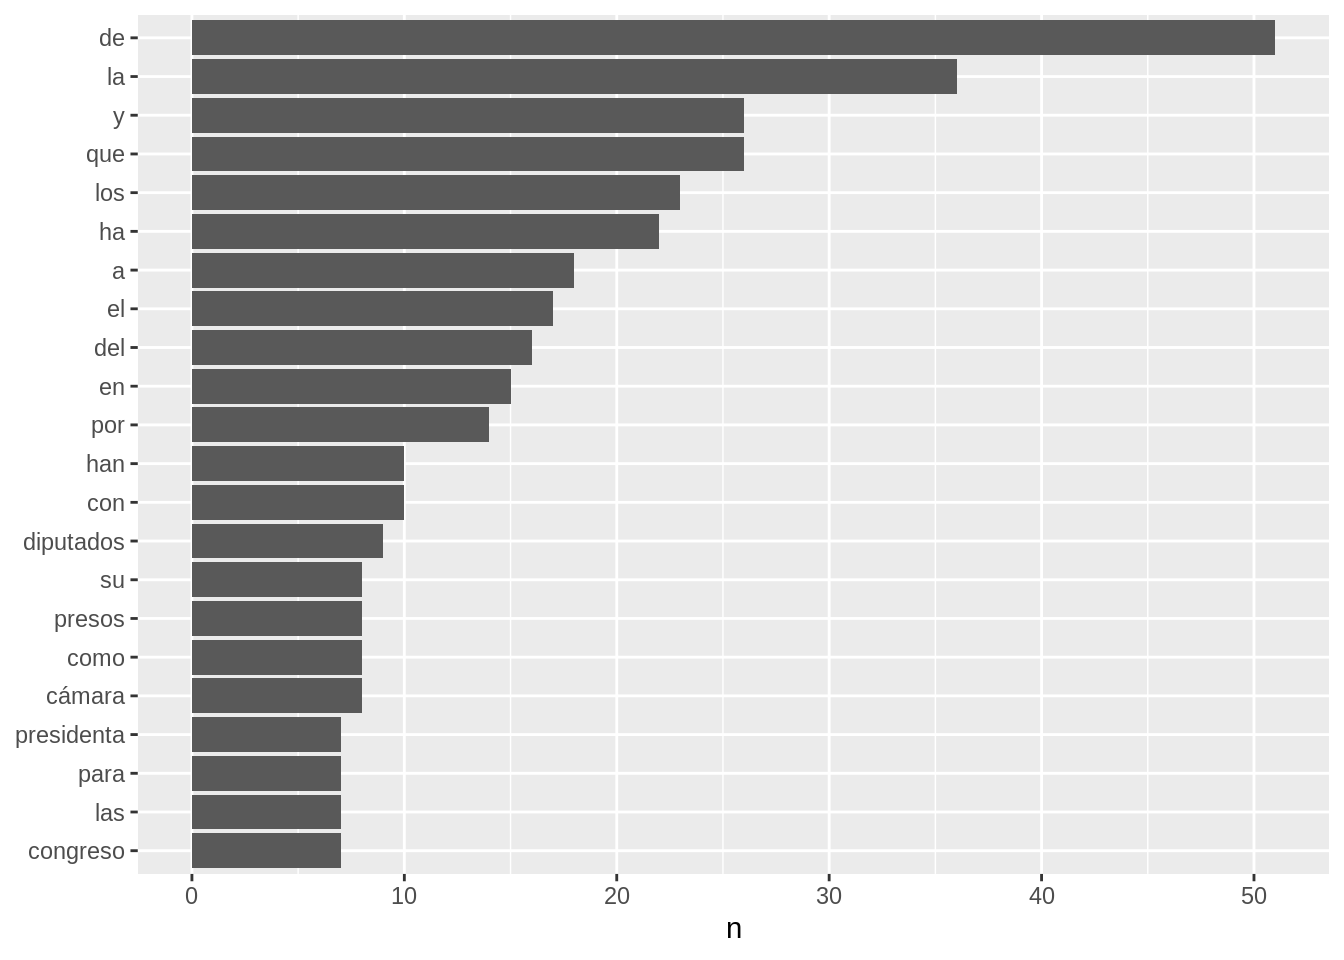
\includegraphics{textRank_files/figure-latex/unnamed-chunk-4-1.pdf}

ahora tenemos todas las entradas suficientes para la función
textrank\_sentences. Sin embargo, iremos un paso más allá y eliminaremos
las palabras de stop en article\_words ya que aparecerían en la mayoría
de las frases y realmente no contienen ninguna información en sí mismas.

\begin{Shaded}
\begin{Highlighting}[]
\NormalTok{article_words <-}\StringTok{ }\NormalTok{article_words }\OperatorTok
\StringTok{  }\KeywordTok{anti_join}\NormalTok{(}\KeywordTok{data_frame}\NormalTok{(}\DataTypeTok{word =} \KeywordTok{stopwords}\NormalTok{(}\DataTypeTok{kind =} \StringTok{"es"}\NormalTok{)), }\DataTypeTok{by =} \StringTok{"word"}\NormalTok{)}
\end{Highlighting}
\end{Shaded}

\begin{verbatim}
## Warning: `data_frame()` is deprecated, use `tibble()`.
## This warning is displayed once per session.
\end{verbatim}

Si volvemos a visualizar el gráfico anterior podemos observar como hemos
eliminado las palabras que no aportaban valor a las frases, tales como
los artículos y conjunciones.

\begin{Shaded}
\begin{Highlighting}[]
\NormalTok{article_words }\OperatorTok
\StringTok{  }\KeywordTok{count}\NormalTok{(word, }\DataTypeTok{sort =} \OtherTok{TRUE}\NormalTok{) }\OperatorTok
\StringTok{  }\KeywordTok{filter}\NormalTok{(n }\OperatorTok{>}\StringTok{ }\DecValTok{4}\NormalTok{) }\OperatorTok
\StringTok{  }\KeywordTok{mutate}\NormalTok{(}\DataTypeTok{word =} \KeywordTok{reorder}\NormalTok{(word, n)) }\OperatorTok
\StringTok{  }\KeywordTok{ggplot}\NormalTok{(}\KeywordTok{aes}\NormalTok{(word, n)) }\OperatorTok{+}
\StringTok{  }\KeywordTok{geom_col}\NormalTok{() }\OperatorTok{+}
\StringTok{  }\KeywordTok{xlab}\NormalTok{(}\OtherTok{NULL}\NormalTok{) }\OperatorTok{+}
\StringTok{  }\KeywordTok{coord_flip}\NormalTok{()}
\end{Highlighting}
\end{Shaded}

\includegraphics{textRank_files/figure-latex/unnamed-chunk-6-1.pdf}
Ejecutamos el algoritmo TextRank sólo requiere 2 entradas.

\emph{Un marco de datos con frases }Un data.frame con tokens (en nuestro
caso palabras) que forman parte de cada frase. Así que estamos listos
para correr

\begin{Shaded}
\begin{Highlighting}[]
\NormalTok{article_summary <-}\StringTok{ }\KeywordTok{textrank_sentences}\NormalTok{(}\DataTypeTok{data =}\NormalTok{ article_sentences, }
                                      \DataTypeTok{terminology =}\NormalTok{ article_words)}
\NormalTok{article_summary}
\end{Highlighting}
\end{Shaded}

\begin{verbatim}
## Textrank on sentences, showing top 5 most important sentences found:
##   1. meritxell batet, elegida nueva presidenta del congreso de los diputados  cámara alta.
##   2. ahora entendemos por qué los golpistas querían una presidenta del congreso como ésta y un presidente del gobierno como pedro sánchez que les dejan las manos libres", ha añadido.tanto pp como cs han exigido a la presidenta de la cámara que reúna de inmediato la mesa del congreso para proceder a la suspensión de los cuatro diputados que se encuentran en prisión preventiva.
##   3. "los independentistas han utilizado la cámara para dar un mitin y la presidenta del congreso ha sido cómplice", ha dicho casado para quien varios diputados "han ultrajado la cámara, la soberanía nacional y la democracia".
##   4. batet ha dado por hecho que todos los parlamentarios han prometido la carta magna acomodándose a los términos que prevé el tribunal constitucional.sin embargo, las fórmulas que han empleado los diputados independentistas para perfeccionar su condición de representantes de una soberanía nacional que rechazan de plano han sido todo un ejemplo de impostura política, de triquiñuela semántica, de puro trampantojo: "por la libertad de los presos y exiliados políticos, por la república catalana y por imperativo legal, prometo", ha dicho gabriel rufián en medio de la algarabía.
##   5. hoy hemos tenido que soportar que algunos diputados utilizaran la expresión presos políticos y sin que la presidenta de la cámara aplicara el reglamento, artículo 103, como es su obligación.
\end{verbatim}

Si bien el método de impresión es bueno, podemos extraer la información
para un buen análisis posterior. La información sobre las frases se
almacena en frases. Incluye la información article\_sentences más la
puntuación de textrank calculada. Si miramos el artículo a lo largo del
tiempo, sería interesante ver dónde aparecen las frases importantes. En
el gráfico siguiente podemos observa que frases poseenmayor score.

\begin{Shaded}
\begin{Highlighting}[]
\NormalTok{article_summary[[}\StringTok{"sentences"}\NormalTok{]] }\OperatorTok
\StringTok{  }\KeywordTok{ggplot}\NormalTok{(}\KeywordTok{aes}\NormalTok{(textrank_id, textrank, }\DataTypeTok{fill =}\NormalTok{ textrank_id)) }\OperatorTok{+}
\StringTok{  }\KeywordTok{geom_col}\NormalTok{() }\OperatorTok{+}
\StringTok{  }\KeywordTok{theme_minimal}\NormalTok{() }\OperatorTok{+}
\StringTok{  }\KeywordTok{scale_fill_viridis_c}\NormalTok{() }\OperatorTok{+}
\StringTok{  }\KeywordTok{guides}\NormalTok{(}\DataTypeTok{fill =} \StringTok{"none"}\NormalTok{) }\OperatorTok{+}
\StringTok{  }\KeywordTok{labs}\NormalTok{(}\DataTypeTok{x =} \StringTok{"Sentence"}\NormalTok{,}
       \DataTypeTok{y =} \StringTok{"TextRank score"}\NormalTok{)}
\end{Highlighting}
\end{Shaded}

\includegraphics{textRank_files/figure-latex/unnamed-chunk-8-1.pdf}


\end{document}
